\subsection{Problem 3.2. More Transportation Schedules}

\begin{figure}[H]
	\centering
%	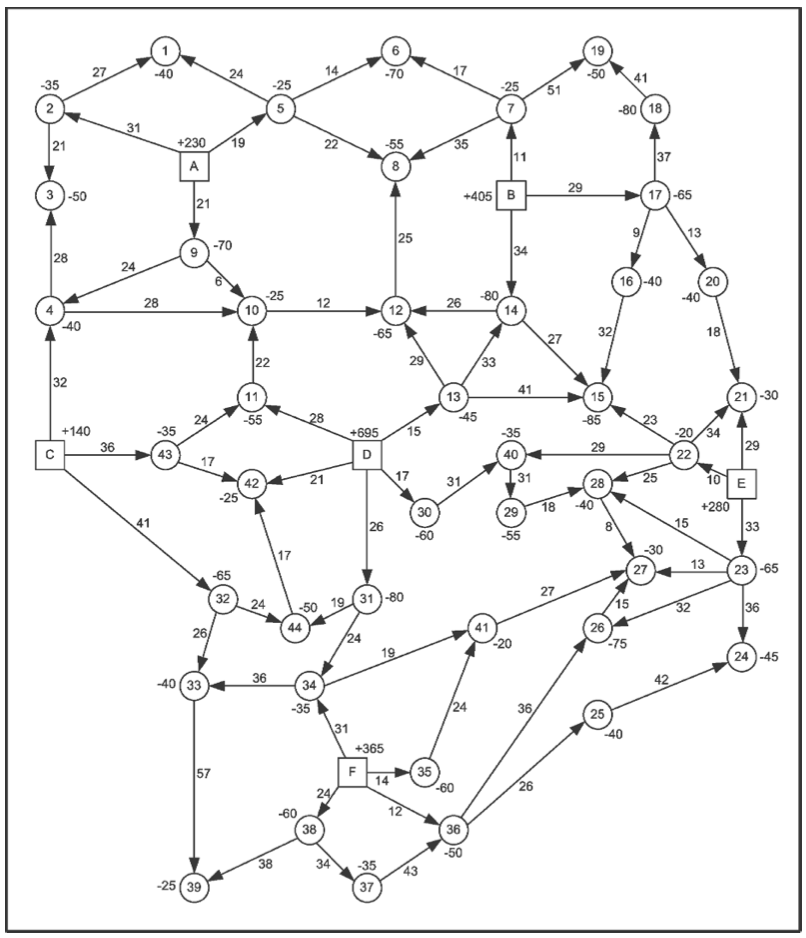
\includegraphics[scale=1]{./img/figure3-14.png}
	\caption{Supplies and demands (in units of 10 spools), and truck costs (in units of \texteuro 10) on a road map with 50 locations}
	\label{network3-2}
\end{figure}

\paragraph{}
\begin{quote}
In another country GTC has to deal with similar questions as in Problem 3.1. In Figure \ref{network3-2} the road map for this country is depicted with 50 locations. There are six cable depots, labeled A, B, C, D, E, and F. All numbers in this figure are given in units of ten spools. The inventories at the various depots are the positive numbers next to the depot labels. For instance, in depot C there are 1,400 cable spools in stock. The locations with labels 1,~\dots,~44 are points where cable is needed, so called demand locations. The numbers next to these labels (with a negative sign) refer to the number of spools demanded at these points. For instance, 650 spools needed at location 17. The numbers attached to the road segments are the transportation costs (in \texteuro 10 units). For instance, the cost of transporting ten spools with one truck is \texteuro 290 on the road segment 22 $\rightarrow$ 40.
\end{quote}

